\documentclass[a4paper,12pt]{extarticle}
\usepackage{geometry}
\usepackage[T1]{fontenc}
\usepackage[utf8]{inputenc}
\usepackage[english,russian]{babel}
\usepackage{amsmath}
\usepackage{amsthm}
\usepackage{amssymb}
\usepackage{fancyhdr}
\usepackage{setspace}
\usepackage{graphicx}
\usepackage{colortbl}
\usepackage{tikz}
\usepackage{pgf}
\usepackage{subcaption}
\usepackage{listings}
\usepackage{indentfirst}
\usepackage[
backend=biber,
style=numeric,
maxbibnames=99
]{biblatex}
\addbibresource{refs.bib}
\usepackage[colorlinks,citecolor=blue,linkcolor=blue,bookmarks=false,hypertexnames=true, urlcolor=blue]{hyperref} 
\usepackage{indentfirst}
\usepackage{mathtools}
\usepackage{booktabs}
\usepackage[flushleft]{threeparttable}
\usepackage{tablefootnote}

\usepackage{chngcntr} % нумерация графиков и таблиц по секциям
\counterwithin{table}{section}
\counterwithin{figure}{section}

\graphicspath{{graphics/}}%путь к рисункам

\makeatletter
% \renewcommand{\@biblabel}[1]{#1.} % Заменяем библиографию с квадратных скобок на точку:
\makeatother

\geometry{left=2.5cm}% левое поле
\geometry{right=1.0cm}% правое поле
\geometry{top=2.0cm}% верхнее поле
\geometry{bottom=2.0cm}% нижнее поле
\setlength{\parindent}{1.25cm}
\renewcommand{\baselinestretch}{1.5} % междустрочный интервал


\newcommand{\bibref}[3]{\hyperlink{#1}{#2 (#3)}} % biblabel, authors, year
\addto\captionsrussian{\def\refname{Список литературы (или источников)}} 

\renewcommand{\theenumi}{\arabic{enumi}}% Меняем везде перечисления на цифра.цифра
\renewcommand{\labelenumi}{\arabic{enumi}}% Меняем везде перечисления на цифра.цифра
\renewcommand{\theenumii}{.\arabic{enumii}}% Меняем везде перечисления на цифра.цифра
\renewcommand{\labelenumii}{\arabic{enumi}.\arabic{enumii}.}% Меняем везде перечисления на цифра.цифра
\renewcommand{\theenumiii}{.\arabic{enumiii}}% Меняем везде перечисления на цифра.цифра
\renewcommand{\labelenumiii}{\arabic{enumi}.\arabic{enumii}.\arabic{enumiii}.}% Меняем везде перечисления на цифра.цифра

\begin{document}
\begin{titlepage}
\newpage

\begin{center}
FEDERAL STATE AUTONOMOUS EDUCATIONAL INSTITUTION FOR\\
HIGHER PROFESSIONAL EDUCATION NATIONAL RESEARCH\\
UNIVERSITY\\
«HIGHER SCHOOL OF ECONOMICS»\\
\bigskip
Faculty of Computer Science
\end{center}

\vspace{2em}

\begin{center}
\underline{Marozau Leu}
\end{center}

\vspace{2em}

\begin{center}
Обнаружение эмоций на основе текста
\end{center}

\vspace{2em}

\begin{center}
Text-Based Emotion Detection
\end{center}

\vspace{4em}

\begin{center}
Qualification paper — Master of Science Dissertation\\
Field of study 01.04.02 «Applied Mathematics and Informatics»\\
Program: 
\end{center}

\vspace{6em}

\begin{flushleft}
Student\\
Marozau Leu
\end{flushleft}

\vspace{4em}

\begin{flushright}
Supervisor\\
Shirnin Alexander Andreevich
\end{flushright}

\vspace{\fill}

\begin{center}
Moscow, 2025
\end{center}

\end{titlepage}
% это титульный лист - выберите подходящий вам из имеющихся в проекте вариантов (kr - курсовая работа у 3 курса, vkr - выпускная квалификационная работа у 4 курса)
\newpage
\setcounter{page}{2}

{
	\hypersetup{linkcolor=black}
	\tableofcontents
}

\newpage

\section*{Abstract}

This thesis explores various approaches for multi-label emotion detection in text across multiple languages. We investigate traditional supervised approaches including BERT, SetFit, and Seq2Seq models, as well as a novel retrieval-augmented generation system called EmoRAG. Using the BRIGHTER dataset, which covers 28 languages including many low-resource ones, we demonstrate that our EmoRAG system achieves state-of-the-art performance without requiring extensive model training. This work contributes to the field of multilingual emotion recognition by providing a comparative analysis of different approaches and introducing an efficient, scalable method for detecting emotions across diverse languages.

\addcontentsline{toc}{section}{Abstract}

\section*{Keywords}
Deep learning, emotion detection, multilingual NLP, retrieval-augmented generation, low-resource languages, multi-label classification

\section{Introduction}

Emotions are fundamental to human communication and experience, coloring our interactions, decisions, and perceptions. The ability to detect and understand emotions in text has become increasingly important in natural language processing (NLP), with applications spanning various domains including customer service, mental health monitoring, content recommendation, social media analysis, and educational technology.

Unlike traditional sentiment analysis, which typically focuses on determining whether a text is positive, negative, or neutral, emotion detection aims to identify specific emotional states such as joy, sadness, anger, fear, surprise, and disgust. This fine-grained understanding of affective content enables more nuanced and human-like interactions between computational systems and users.

The development of effective multi-lingual, multi-label emotion detection systems faces several interconnected challenges. Linguistic diversity presents a significant hurdle, as human languages vary dramatically in their lexical, syntactic, and semantic structures, including how emotions are expressed. Data scarcity is particularly problematic for low-resource languages, which lack substantial labeled datasets for emotion detection. The multi-label nature of emotions adds complexity, as texts frequently express multiple emotions simultaneously. Cross-cultural variations in how emotions are expressed and interpreted further complicate the development of universally applicable systems. Finally, computational efficiency concerns arise when considering the impracticality of training separate models for thousands of languages.

This thesis investigates multi-lingual, multi-label emotion detection, exploring approaches that can operate effectively with limited labeled data, adapt to linguistic and cultural differences, and handle the inherent complexity of multi-label emotion classification. We compare traditional supervised approaches with newer paradigms like retrieval-augmented generation, examining their effectiveness across languages with varying resource availability.

The remainder of this thesis is organized as follows:

\textbf{Chapter 2: Related Work} reviews previous research in emotion detection, multi-label classification, multi-lingual NLP models, retrieval-augmented generation, few-shot learning, and large language models for emotion detection.

\textbf{Chapter 3: Data} describes the BRIGHTER dataset, including its creation, annotation process, and composition.

\textbf{Chapter 4: Methodology} presents our four approaches: BERT-based fine-tuning, SetFit few-shot learning, Seq2Seq generative models, and our novel EmoRAG system.

\textbf{Chapter 5: Experiments} outlines our experimental setup, evaluation metrics, and hyperparameter tuning strategies.

\textbf{Chapter 6: Results} analyzes our experimental findings, including performance comparisons across approaches, languages, and emotion categories.

\textbf{Chapter 7: Discussion} interprets our results, comparing the strengths and weaknesses of each approach.

\textbf{Chapter 8: Conclusion and Future Work} summarizes key findings and suggests directions for future research.

\section{Related Work}

This chapter reviews key literature relevant to multi-lingual, multi-label emotion detection, focusing on four areas: traditional approaches to emotion detection, multi-label classification techniques, large language models, and retrieval-augmented generation systems.

\subsection{Emotion Detection in Text}

Emotion detection in text has evolved significantly over the past two decades. Early work by \cite{strapparava2007semeval} introduced one of the first datasets for emotion recognition in English text, defining the task as detecting Ekman's six basic emotions: joy, sadness, anger, fear, surprise, and disgust. This work established the foundation for most subsequent research in the field.

Classical approaches to emotion detection included lexicon-based methods and traditional machine learning techniques. \cite{mohammad2013crowdsourcing} developed the NRC Emotion Lexicon, mapping English words to emotions. These approaches provide strong baselines but struggle with contextual understanding and required extensive manual annotation for each language.

The advent of deep learning brought significant advances to emotion detection. \cite{felbo2017using} introduced DeepMoji, leveraging distant supervision from emojis to pre-train models for emotion recognition. More recently, transformer-based approaches have set new benchmarks. \cite{demszky2020goemotions} created GoEmotions, a large-scale dataset with 27 emotion categories, and demonstrated strong performance with BERT-based models.

\subsection{Multi-label Classification and Language Models}

Multi-label classification, where instances can belong to multiple categories simultaneously, is inherently relevant to emotion detection as texts often express multiple emotions at once. 

Classical approaches to multi-label classification include binary relevance, which trains independent classifiers for each label, and label powerset, which transforms the problem into a multi-class classification task with each unique label combination as a separate class. \cite{read2011classifier} introduced classifier chains, which model inter-label dependencies by building a sequence of binary classifiers, demonstrating significant improvements over binary relevance methods.

The evolution of language models has dramatically impacted text classification tasks, including emotion detection. BERT \cite{devlin2019bert} and its multilingual variant mBERT demonstrated strong performance across languages and tasks through contextual representations and pre-training on massive corpora. XLM-RoBERTa \cite{conneau2020unsupervised} further improved cross-lingual capabilities by training on 100 languages with 2.5 times more data than mBERT.

Large Language Models (LLMs) like GPT-3 \cite{brown2020language} and its successors have shown remarkable few-shot capabilities through in-context learning, where models make predictions based on examples provided in the prompt. This paradigm shift has significant implications for multi-lingual emotion detection, potentially reducing the need for extensive labeled data in each language.

For multi-label settings, deep learning approaches have shown promise. \cite{nam2014large} demonstrated that using cross-entropy loss with a sigmoid activation function per label outperforms ranking-based loss functions in neural networks. 

\subsection{Few-shot Learning in NLP}

Few-shot learning has become increasingly important for addressing data scarcity in NLP, particularly for low-resource languages. \cite{brown2020language} demonstrated the remarkable few-shot capabilities of large language models through in-context learning, where a model makes predictions based on a few examples provided in the prompt.

Building on this foundation, \cite{gao2021making} showed that carefully constructed prompts with strategically selected examples can dramatically improve few-shot performance on various NLP tasks, including classification. For more specialized applications, \cite{tunstall2022efficient} developed SetFit, a few-shot learning approach that combines contrastive learning with classification fine-tuning. By leveraging sentence transformers and efficient pair-wise training, SetFit achieves strong performance with as few as 8 examples per class.

The selection of examples for few-shot learning significantly impacts performance. \cite{liu2022few} showed that retrieving examples based on semantic similarity to the test instance outperforms random selection, especially for complex tasks. Cross-lingual few-shot learning presents additional challenges. 

Despite these advances, few-shot learning in multi-label settings remains challenging. \cite{hou2022few} addressed this gap with a specialized few-shot learning approach for multi-label classification that captures label correlations even with limited examples.

\subsection{Retrieval-Augmented Generation (RAG)}

Retrieval-Augmented Generation (RAG) has emerged as a powerful paradigm for enhancing language model capabilities with external knowledge. \cite{lewis2020retrieval} introduced the original RAG framework, combining dense retrieval with sequence-to-sequence models to generate outputs conditioned on relevant retrieved documents.

While RAG was initially developed for generation tasks, its application to classification has shown promising results. \cite{gao2024retrieval} adapted RAG for text classification, demonstrating that retrieved examples can serve as few-shot demonstrations to guide in-context learning. Their approach achieved competitive performance on various classification benchmarks without requiring task-specific fine-tuning.

For multi-lingual contexts, \cite{shi2023replug} developed Cross-Lingual RAG, which leverages a shared dense retrieval space across languages to retrieve relevant documents for low-resource languages. This approach is particularly valuable for emotion detection across diverse languages, as it enables knowledge transfer from high-resource to low-resource languages.

The selection of retrieved documents significantly impacts RAG performance. \cite{gao2023retrieval} introduced techniques for dynamic retrieval that adapt to the specific needs of each query, showing that adaptive retrieval strategies outperform static approaches. In classification contexts, \cite{singh2022flare} demonstrated that RAG can mitigate the challenge of domain shift by retrieving examples similar to the test instance, regardless of their source domain.

\subsection{Research Gaps and Opportunities}

Our review of the literature reveals several important gaps that this thesis aims to address:

\begin{enumerate}

    \item \textbf{Few-shot Learning for Low-resource Languages}: Most emotion detection systems require substantial labeled data, which is unavailable for many languages. Few studies have explored how large language models can effectively perform emotion detection with minimal examples across diverse languages.
    
    \item \textbf{Ensemble Methods for Multi-label Emotion Detection}: While ensemble approaches have shown promise in various NLP tasks, their application to multi-label emotion detection, particularly in multi-lingual settings, remains underexplored. There is limited research on how to effectively combine multiple LLM predictions to improve performance across emotions and languages.
    
    \item \textbf{Retrieval-Augmented Classification}: While RAG has shown promise for generation tasks, its application to multi-label classification, particularly emotion detection, remains underexplored.

    \item \textbf{Balancing Performance Across Languages}: Existing approaches often show significant performance disparities between high-resource and low-resource languages. Few studies have systematically addressed how to design systems that maintain consistent performance across linguistically diverse languages.
    
    \item \textbf{Low-Resource Adaptability}: Few studies have explicitly addressed how emotion detection approaches can be adapted for low-resource languages with minimal labeled data.

    \item \textbf{Capturing Emotion Co-occurrence Patterns}: The multi-label nature of emotion detection presents unique challenges, as emotions often co-occur in complex patterns. Limited research exists on how few-shot LLM approaches can effectively model these interdependencies without extensive training data.
    
\end{enumerate}

\section{Data}
\subsection{Overview}

\begin{figure}[h]
    \centering
    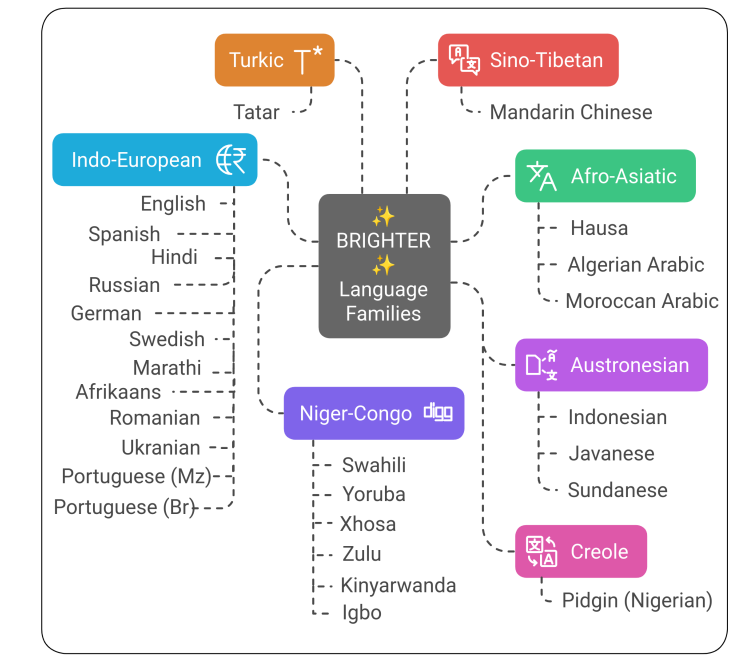
\includegraphics[width=0.5\textwidth]{brighter_languages.png}
    \caption{Languages in the BRIGHTER dataset}
    \label{fig:brighter_languages}
\end{figure}

\begin{figure}[h]
    \centering
    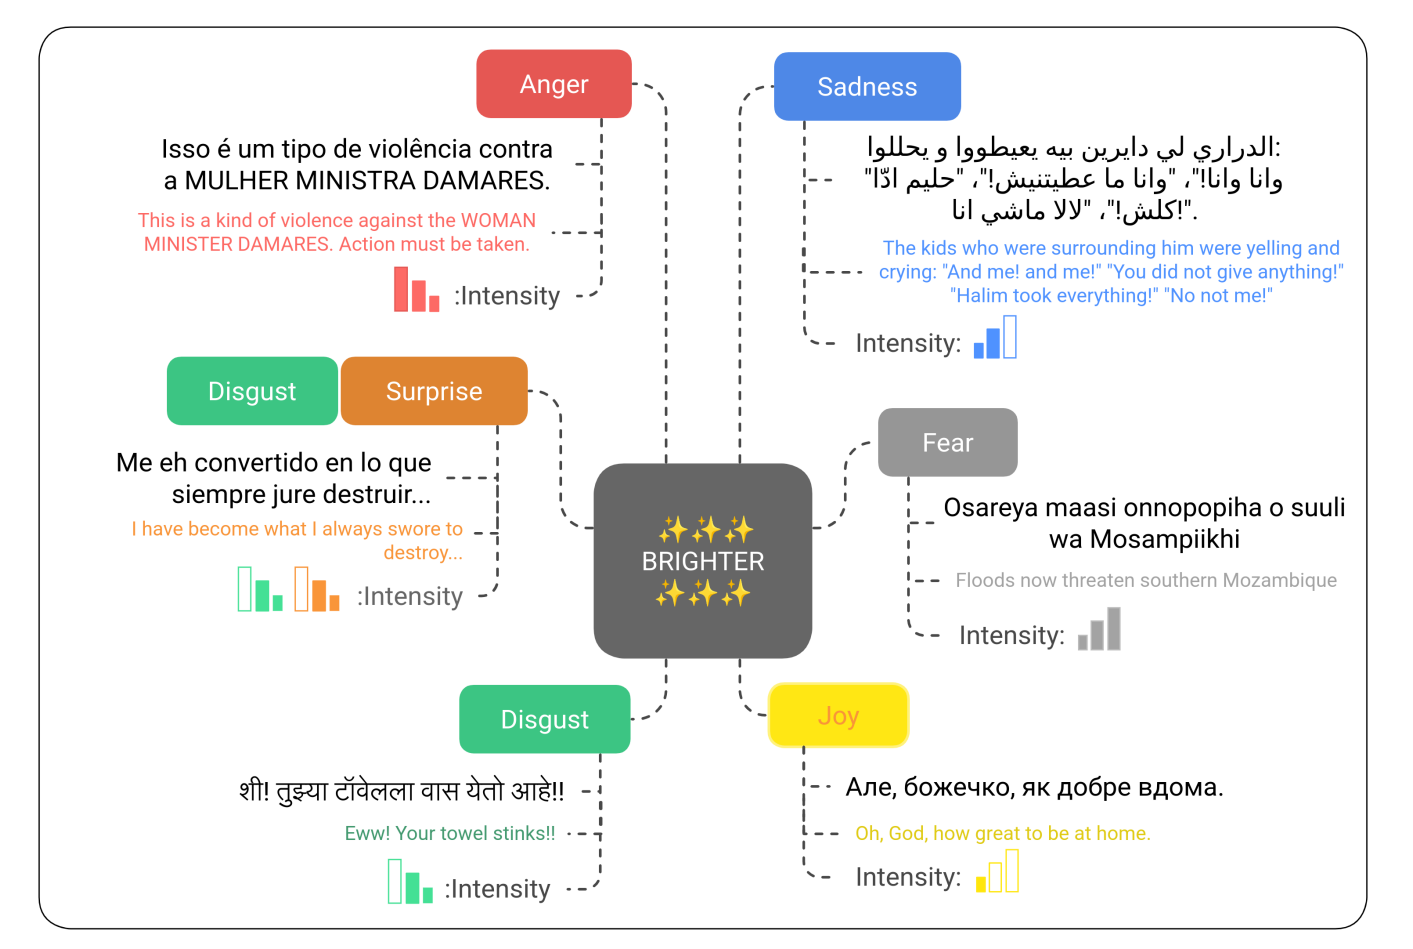
\includegraphics[width=0.8\textwidth]{brighter_examples.png}
    \caption{Examples from the BRIGHTER dataset}
    \label{fig:brighter_examples}
\end{figure}

The BRIGHTER dataset \cite{muhammad2025brighterbridginggaphumanannotated} is a comprehensive, multi-labeled, multilingual resource for textual emotion recognition, consisting of over 100,000 annotated examples across 28 languages and 7 language families. Designed to address the stark resource imbalance in emotion research, BRIGHTER prioritizes low-resource languages from Africa, Asia, Eastern Europe, and Latin America, while also including mid- and high-resource languages such as English, German, and Portuguese.

Each instance in BRIGHTER is manually annotated by fluent speakers, with annotations covering six core perceived emotions — \textit{joy}, \textit{sadness}, \textit{anger}, \textit{fear}, \textit{surprise}, and \textit{disgust} — and includes an additional \textit{neutral} label when no emotion is expressed. Annotations are multi-label and span four emotion intensity levels (0 to 3).

The dataset aggregates data from diverse sources, including social media platforms (e.g., Reddit, YouTube, Weibo), speeches, literature, news, and even machine-generated examples with human post-editing. A detailed breakdown of these sources, annotator counts, and splits per language is given in the original BRIGHTER paper, with representative examples shown in Figure~\ref{fig:brighter_examples} and the language family distribution illustrated in Figure~\ref{fig:brighter_languages}.

\subsection{Data Splits}
We use the official BRIGHTER dataset splits for all experiments:

\begin{itemize}
\item \textbf{Training Set}: Approximately 70\% of the data, used for supervised model training.
\item \textbf{Validation Set}: Approximately 15\% of the data, used for early stopping and hyperparameter tuning.
\item \textbf{Test Set}: Approximately 15\% of the data, reserved for final evaluation.
\item \textbf{Development Set}: A curated subset drawn from training and validation sets, used to construct few-shot examples.
\end{itemize}

To ensure fair evaluation across the linguistic spectrum, we applied stratified sampling for low-resource languages, preserving both emotion and language distributions during splitting.

\subsection{Dataset Challenges}

\begin{figure}[h]
    \centering
    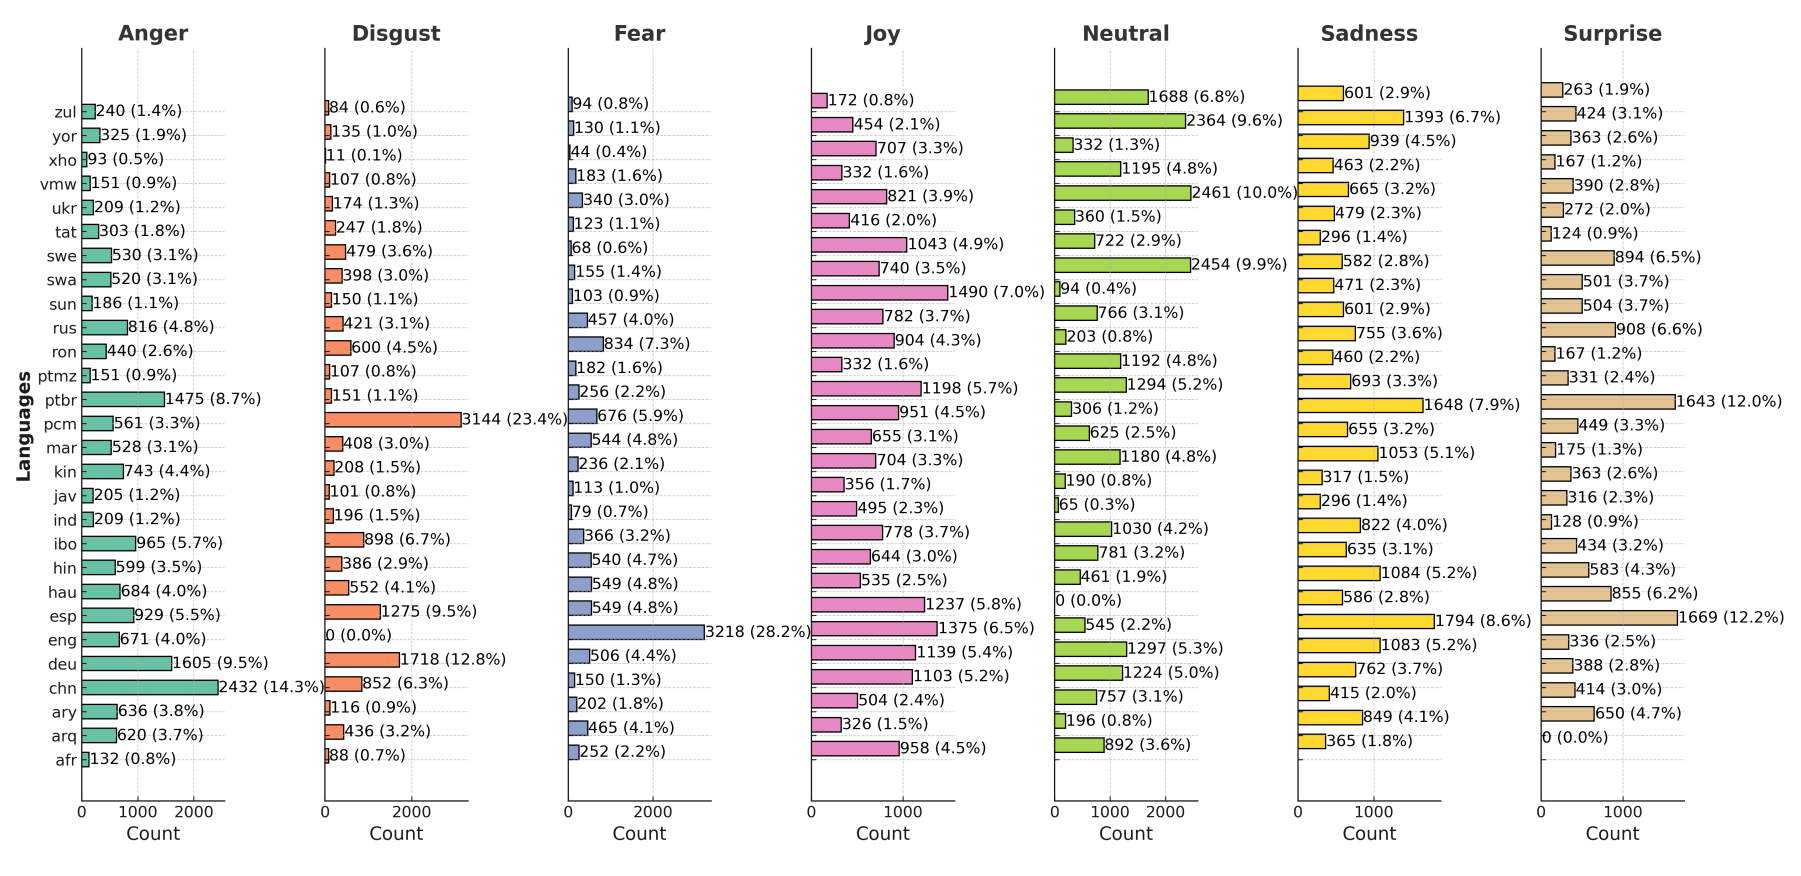
\includegraphics[width=1\textwidth]{brighter_label_distribution.png}
    \caption{Label distribution in the BRIGHTER dataset}
    \label{fig:brighter_label_distribution}
\end{figure}

While BRIGHTER is a rich and diverse resource, it also introduces several challenges that motivated our modeling choices:

Label Distribution: The dataset exhibits long-tailed distributions for both emotions and languages, as illustrated in Figure~\ref{fig:brighter_label_distribution}. Some languages lack examples for certain emotions (e.g., no \textit{disgust} in English, no \textit{surprise} in Afrikaans), and neutral examples vary greatly in frequency.

Linguistic Coverage: BRIGHTER spans typologically diverse languages with varying scripts (Latin, Arabic, Devanagari, Cyrillic), making it a strong benchmark for cross-lingual generalization.

Annotation Density: Most languages have between 3 and 10 annotators per example, but annotation intensity and agreement levels vary. Final labels were aggregated using a combination of per-emotion thresholding and average intensity, ensuring consistent quality across languages.

These considerations led us to explore both supervised and retrieval-augmented methods, with the aim of improving generalization under low-resource, high-diversity conditions.

\section{Methodology}

This chapter presents the various approaches we explored for multi-lingual, multi-label emotion detection using the BRIGHTER dataset. We investigate both traditional supervised learning approaches (BERT, SetFit, and Seq2Seq) and a novel retrieval-augmented generation (RAG) approach called EmoRAG. Each approach represents a different paradigm in machine learning for text classification:

\begin{enumerate}
\item \textbf{BERT-based Approach}: Fine-tune a pre-trained language model with a classification head for multi-label prediction
\item \textbf{SetFit Approach}: A few-shot learning technique that combines contrastive learning with standard classification techniques
\item \textbf{Seq2Seq Approach}: Framing emotion detection as a text generation task
\item \textbf{EmoRAG System}: A novel retrieval-augmented generation system that leverages few-shot learning without parameter updates
\end{enumerate}

The following sections describe each approach in detail, including model architecture, training procedures, and implementation specifics.

\subsection{BERT-based Approach}

For prediction, we apply a sigmoid function to the model outputs and use a threshold of 0.5 to convert probabilities to binary predictions:

Performance is evaluated using F1-micro and F1-macro metrics, which are particularly suitable for multi-label classification with imbalanced classes.

The BERT-based approach provides a strong baseline for emotion detection, leveraging the powerful contextual representations of transformer models. However, it may struggle with low-resource languages where pre-training data is limited.

\subsection{SetFit Approach}

SetFit (Sentence Transformer Fine-tuning) is a novel few-shot learning method introduced by \cite{tunstall2022efficient} that combines contrastive learning with standard classification techniques. It was designed to achieve strong performance with limited labeled data, making it particularly suitable for multi-lingual emotion detection where labeled examples may be scarce for low-resource languages.

\subsubsection{SetFit Overview}

The SetFit approach consists of two main stages:

\begin{enumerate}
\item \textbf{Contrastive Learning Stage}: Fine-tune a sentence transformer model using contrastive learning on sentence pairs derived from labeled examples.
\item \textbf{Classification Stage}: Train a classifier (typically a linear model) on the embeddings produced by the fine-tuned sentence transformer.
\end{enumerate}

Figure~\ref{fig:setfit_training} illustrates the SetFit training process.

\begin{figure}[h]
    \centering
    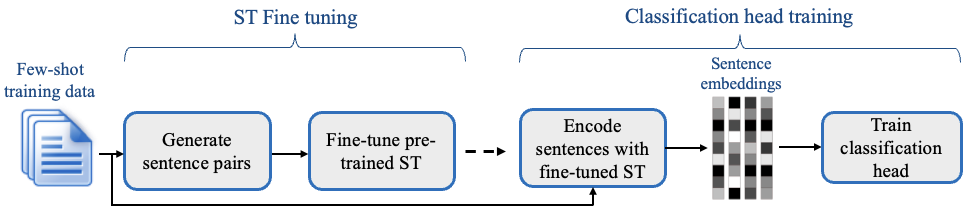
\includegraphics[width=0.8\textwidth]{setfit.png}
    \caption{SetFit training process}
    \label{fig:setfit_training}
\end{figure}

The key innovation of SetFit is its ability to leverage the power of sentence transformers for few-shot learning without requiring extensive labeled data or computationally expensive prompt-based approaches. By fine-tuning the sentence embeddings directly on the task-specific data, SetFit can adapt pre-trained embeddings to better represent the nuances of emotion detection across languages.

\subsection{EmoRAG System}

EmoRAG (Emotion Retrieval-Augmented Generation) is a novel system developed for multi-label emotion detection that reframes the problem through the lens of retrieval-augmented generation. Rather than relying on model fine-tuning, EmoRAG leverages the knowledge captured in labeled examples retrieved at inference time, enabling multilingual, few-shot emotion classification without updating model parameters.

\subsubsection{Pipeline Overview}

The EmoRAG architecture follows a four-stage pipeline, illustrated in Figure~\ref{fig:emorag_pipeline}:

\begin{enumerate}
\item \textbf{Database Construction}: The system first indexes the labeled examples from the BRIGHTER training dataset as a retrieval corpus.
\item \textbf{Retrieval}: An n-gram or embedding-based retriever fetches the top-K most similar examples to a given input.
\item \textbf{Generation}: The retrieved examples are used as few-shot prompts for a set of pre-trained large language models (LLMs) to produce emotion predictions.
\item \textbf{Aggregation}: The individual model predictions are combined via a learned or heuristic aggregation strategy (e.g., majority vote, label-weighted averaging) to produce the final multi-label output.
\end{enumerate}


\begin{figure}[h]
    \centering
    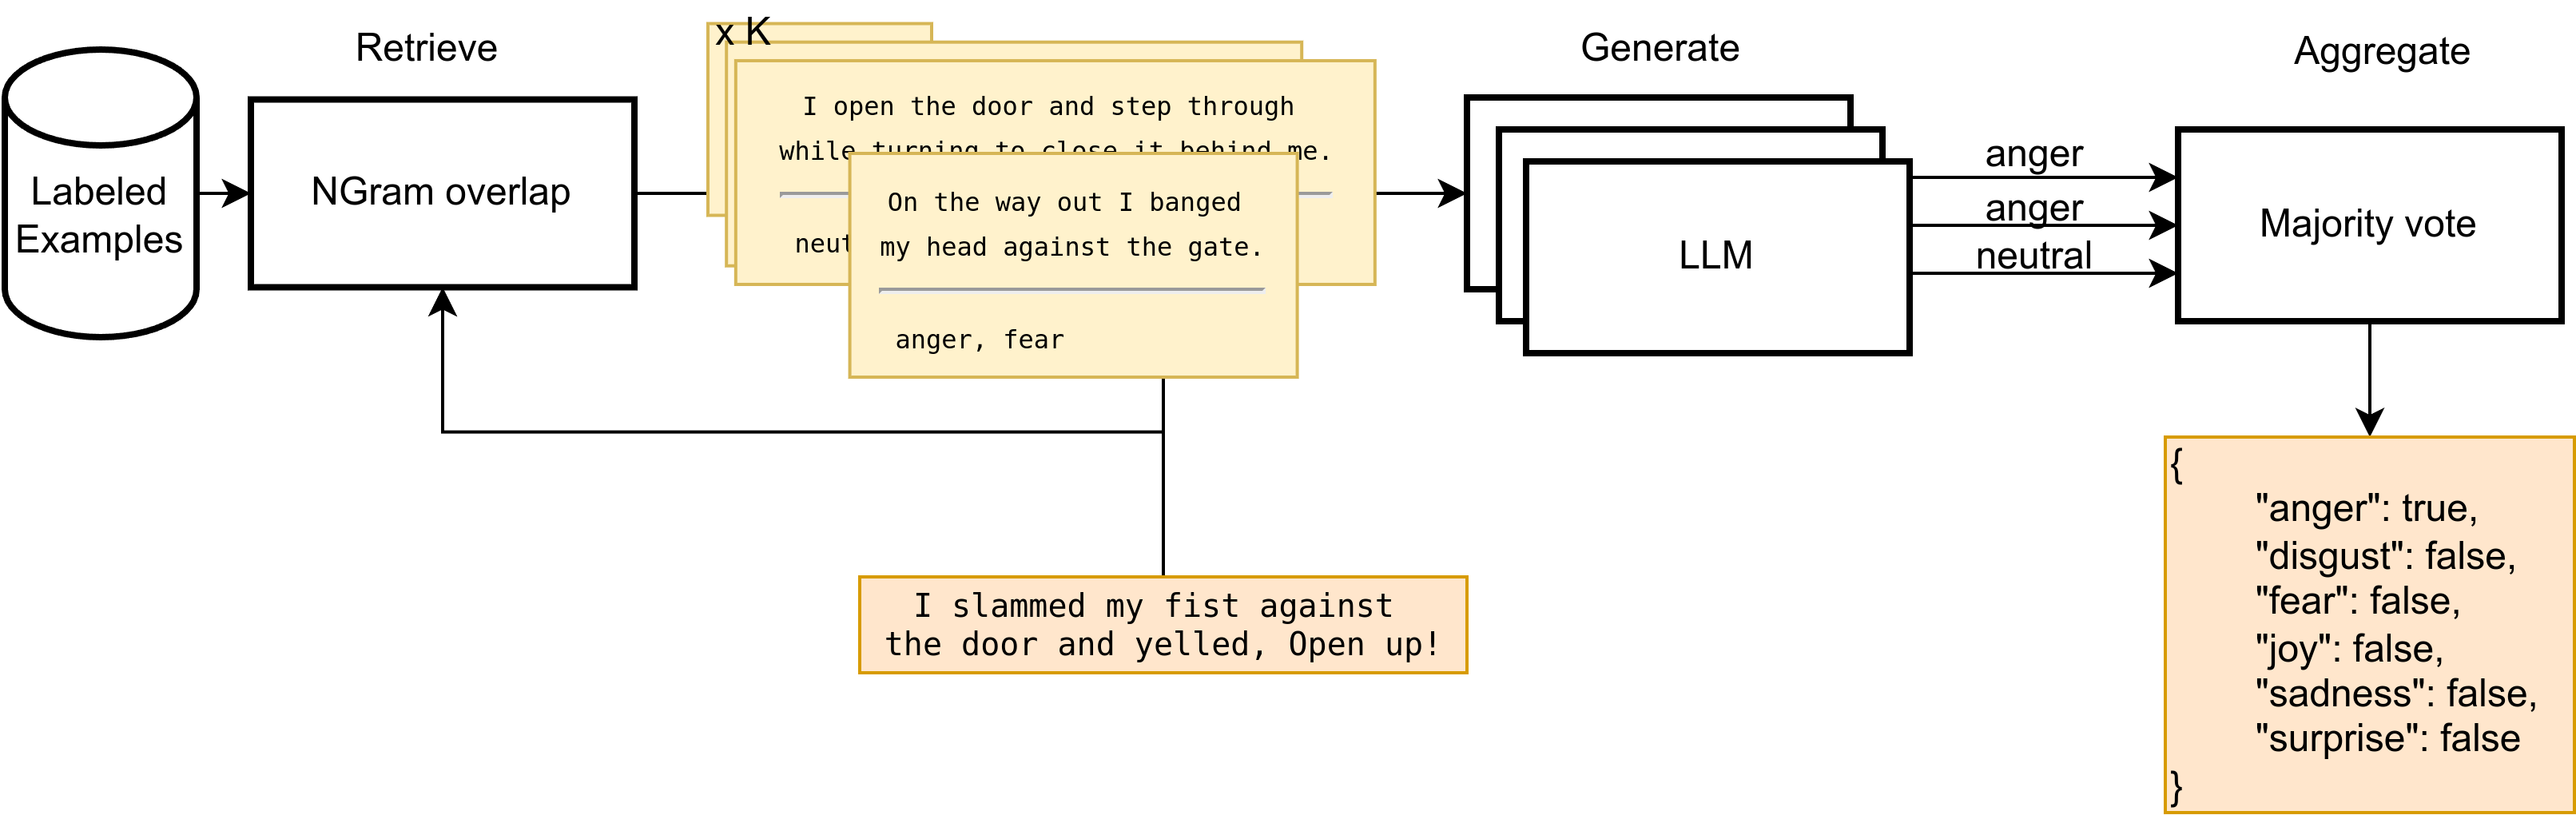
\includegraphics[width=0.8\textwidth]{emorag.png}
    \caption{The EmoRAG pipeline includes a retriever, a set of LLMs, and an aggregation module. Retrieved labeled examples are used as prompts to generate multi-label predictions.}
    \label{fig:emorag_pipeline}
\end{figure}

\subsubsection{Retriever Component}

We experimented with two retrieval strategies:
\begin{itemize}
\item \textbf{N-gram Overlap}: Particularly effective for low-resource languages, this method retrieves examples based on surface lexical similarity.
\item \textbf{Embedding-based Retrieval (BGE-M3)}: A dense vector retriever using sentence-level embeddings that supports multilingual representations.
\end{itemize}

The number of retrieved samples K is fixed per language type: 30 for low-resource languages and 100 for high-resource ones.

\subsubsection{Generator Models}

For generation, EmoRAG uses a diverse ensemble of LLMs including:
\begin{itemize}
\item \texttt{Llama-3.1-70B}
\item \texttt{Qwen2.5-72B-Instruct}
\item \texttt{Gemma-2-27B-it}
\item \texttt{GPT-4o-mini}
\end{itemize}
Each LLM receives the same prompt structure, written in English and formatted to generate emotion predictions in JSON format:
\begin{verbatim}
{
"anger": bool,
"fear": bool,
"joy": bool,
"sadness": bool,
"surprise": bool,
"disgust": bool
}
\end{verbatim}

\subsubsection{Aggregation Strategies}

To aggregate predictions from multiple LLMs, we evaluate five strategies:
\begin{itemize}
\item \textbf{Single model} output (e.g., GPT-4o-mini)
\item \textbf{Majority Vote}
\item \textbf{Macro/Micro-F1 Weighted Voting}
\item \textbf{Label-specific F1 Voting} – the most successful method in our experiments
\item \textbf{LLM-based Aggregation} – using one LLM to aggregate others’ outputs
\end{itemize}


\section{Experiments}

\subsection{Experimental Setup}
\begin{itemize}
\item \textbf{Hardware and Software}: Details on the implementation environment
\item \textbf{Model Configurations}: Specific parameters for each approach
\item \textbf{Training Process}: Time, resources, and optimization techniques
\item \textbf{Cross-validation}: Strategies for ensuring robust evaluation
\end{itemize}

\subsection{Evaluation Metrics}
\begin{itemize}
\item \textbf{F1-micro and F1-macro}: Definition and justification
\item \textbf{Language-specific Evaluation}: How performance is assessed across languages
\item \textbf{Emotion-specific Metrics}: Evaluation for each emotion category
\end{itemize}

\subsection{Hyperparameter Tuning}
\begin{itemize}
\item \textbf{BERT Hyperparameters}: Learning rates, batch sizes, etc.
\item \textbf{SetFit Hyperparameters}: Sampling strategies, example counts, etc.
\item \textbf{Seq2Seq Hyperparameters}: Beam width, repetition penalty, etc.
\item \textbf{EmoRAG Hyperparameters}: Example counts, retrieval mechanisms, etc.
\end{itemize}

\section{Results}

\subsection{Overall Performance}
\begin{itemize}
\item \textbf{Comparative Analysis}: Performance of all approaches
\item \textbf{Statistical Significance}: Analysis of performance differences
\item \textbf{Efficiency Comparison}: Training time, inference time, and resource requirements
\end{itemize}

\subsection{Performance by Language}
\begin{itemize}
\item \textbf{High-resource vs. Low-resource Languages}: Analysis of performance differences
\item \textbf{Language Family Analysis}: Patterns across related languages
\item \textbf{Cross-lingual Transfer}: Evidence of knowledge transfer between languages
\end{itemize}

\subsection{Performance by Emotion}
\begin{itemize}
\item \textbf{Emotion-specific Analysis}: Differences in detection accuracy by emotion
\item \textbf{Co-occurrence Patterns}: Analysis of multi-label predictions
\item \textbf{Confusion Analysis}: Common misclassifications between emotions
\end{itemize}

\subsection{Ablation Studies}
\begin{itemize}
\item \textbf{EmoRAG Components}: Impact of different retrievers, generators, and aggregation strategies
\item \textbf{Example Count Analysis}: Performance vs. number of examples
\item \textbf{Cross-model Analysis}: Contribution of different LLMs to the ensemble
\end{itemize}

\section{Discussion}

\subsection{Comparison of Approaches}
\begin{itemize}
\item \textbf{Strengths and Weaknesses}: Analysis of each approach
\item \textbf{Resource Efficiency}: Trade-offs between performance and computational requirements
\item \textbf{Practical Considerations}: Deployment scenarios for different approaches
\end{itemize}

\subsection{Performance on Low-resource Languages}
\begin{itemize}
\item \textbf{Challenges}: Specific issues in low-resource settings
\item \textbf{Transfer Learning Effects}: How well knowledge transfers to low-resource languages
\item \textbf{Retrieval Benefits}: How retrieval mechanisms help in low-resource scenarios
\end{itemize}

\subsection{Error Analysis}
\begin{itemize}
\item \textbf{Common Error Patterns}: Analysis of misclassifications
\item \textbf{Language-specific Challenges}: Linguistic factors affecting performance
\item \textbf{Cultural Factors}: Impact of cultural differences on emotion expression and detection
\end{itemize}

\section{Conclusion and Future Work}
\begin{itemize}
\item \textbf{Summary of Findings}: Key takeaways from the research
\item \textbf{Limitations}: Constraints and shortcomings of the current approaches
\item \textbf{Future Research Directions}: Promising avenues for further investigation
\item \textbf{Broader Impacts}: Potential applications and implications of the work
\end{itemize}

\printbibliography

\section*{Appendices}
\begin{itemize}
\item \textbf{A. Prompt Templates}: Complete prompts used for LLMs
\item \textbf{B. Hyperparameter Details}: Comprehensive listing of all parameters
\item \textbf{C. Additional Results}: Supplementary tables and figures
\item \textbf{D. Implementation Code}: Links to code repositories
\end{itemize}

\end{document}
